\providecommand{\main}{../../..}
\providecommand{\Figures}{\main/Figures/Micros}

\documentclass[\main/main.tex]{subfiles}

\begin{document}
            
\sectionmark{Le \pz{}, un modèle idéal pour l'imagerie}
\section{La transparence du \pz{} en fait un modèle idéal pour l'imagerie en fluorescence}

\label{sec:imagerie}

Afin d'être par exemple en mesure de détecter les déformations induites par l'exposition d'un \pz{} à un polluant,
ou d'analyser le patron de fluorescence d'une lignée rapportrice,
il est nécessaire d'adapter différents systèmes d'imagerie aux \pz{}.
%
Nous allons donc présenter différents systèmes d'imageries en fluorescence utilisés chez le \pz{}.

    \subsection{La récente diversification des méthodes de microscopie en fluorescence}
    
%% Epifluo
La manière la plus simple d'effectuer une imagerie en fluorescence implique l'épifluorescence.
Ceci consiste à émettre un faisceaux lumineux par le moyen d'une source lumineuse avec un spectre variant de l'infrarouge jusqu'à l'ultraviolet.
%
La sélection de la longueur d'onde désirée pour l'observation se fait simplement par le choix d'un filtre.
%
La simplicité, la rapidité et le faible coût de cette approche la rends particulièrement répandue dans les laboratoires, alors qu'elle présente plusieurs limitations.
%
Son défaut principal est sa forte profondeur de champs.
%
Quelque soit la position du plan focal, le détecteur recevra des photons d'autres positions en Z, ce qui limite fortement la résolution de l'image, même si des post-traitements dits de déconvolution sont effectués.


%% confocal
%
La microscopie confocale par balayage laser est une des premières méthodes d'imagerie ayant été mise au point pour compenser ce défaut. 
%
Brevetée en 1957 (voir \autoref{fig:confocal}), la microscopie confocale repose sur l'utilisation d'une source lumineuse laser et d'un iris.
%
Placé dans le plan focal conjugué de l'objectif utilisé, ce sténopé va empêcher les photons ne se trouvant pas dans le plan focal de l'objectif d'atteindre le détecteur.
%
De cette manière, seuls les photons provenant du plan focal observé retournent au détecteur, ce qui permet d'obtenir une profondeur de champs très faible.
%
Cette dernière sera proportionnelle au diamètre de l'iris. Au minimum, une profondeur de champs d'environ $400 nm$ peut être obtenue.
%
En déplaçant l'objet avec une platine motorisée, il devient alors possible de réaliser des images 3D ayant des résolutions inférieures au micron.
%
La grande précision de cette méthode et la versatilité permise par les méthodes de marquages en ont ainsi fait un outil de choix pour l'étude de phénomènes cellulaires et sub-cellulaires.

\begin{figure}[h!]{\textwidth} 
    \centering
       \centering 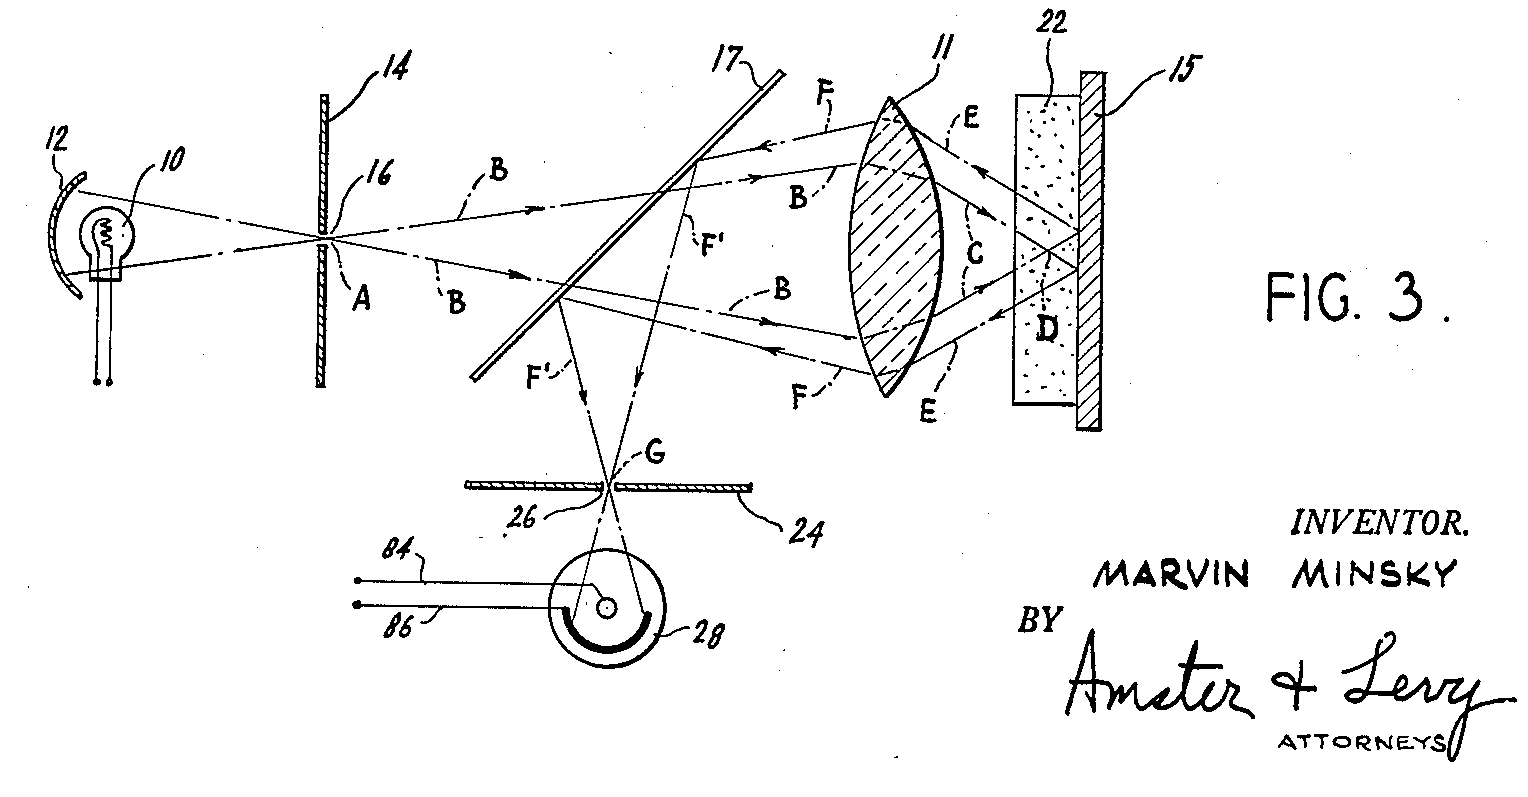
\includegraphics[width=\textwidth]{\Figures/minsky.png}
       \caption{
            \label{fig:confocal}
            Principe de fonctionnement d'un microscope confocale
            \newline
            Le point principal de cette approche consiste à placer le capteur (28) après un iris (26).
            Cet iris va empêcher la captation de photons ne se trouvant pas dans le plan focal de la lentille (11), ce qui permet d'obtenir une très faible profondeur de champ.
            \newline
            Schéma issu du brevet de \textsc{Marvin Minksy} déposé en 1957.
            }
\end{figure}

%
Cependant, cette méthode présente deux défauts majeurs.
%
Premièrement, l'énergie nécessaire pour l'illumination de l'objet est importante, ce qui produit un risque de photo\hyp{}toxicité et de photo\hyp{}blanchiment. Deuxièmement, l'atténuation lumineuse des faisceaux lasers utilisés ne permet pas d'étudier des échantillons épais sans clarification préalable.

%%
%
La microscopie par excitation biphotons améliore la pénétration au sein de l'échantillon.
%
Le concept d'excitation à deux photons est basé sur le fait que pour exciter un électron à un niveau quantique supérieur, plusieurs photons (d’énergie plus basse) peuvent de façon combinée apporter l’énergie nécessaire à l’excitation. Chaque photon transporte environ la moitié de l'énergie nécessaire pour exciter la molécule.Pour que deux photons ayant une forte longueur d'onde et une faible énergie soient en mesure d'exciter un fluorophore, ils doivent être absorbés simultanément. Sans dispositif particulier, la probabilité d'un tel évènement est très faible.  Une excitation entraîne l'émission ultérieure d'un photon de fluorescence. La probabilité d'absorption quasi simultanée de deux photons est extrêmement faible. Par conséquent, une puissance pic élevée de photons d'excitation est généralement requise, ce qui peut généralement être générée par un laser femto\hyp{}seconde.
%%
%
L'utilisation de l'excitation bi-photons présentent plusieurs avantages. Tout d'abord, la réduction de l'énergie des photons infra-rouge émis permet de réduire la photo-toxicité et le photo-blanchiment.
%
La lumière infra-rouge pénètre mieux et diffuse moins dans les tissus, ce qui permet d'imager des tissus plus épais.
%
Cependant, l'utilisation de laser femto\hyp{}secondes implique une forte augmentation des coûts d'achat et de maintenance relativement à l'emploi d'un microscope confocal à balayage laser.


%% SPIM
\label{sec:spim}
Une autre stratégie permettant l'imagerie en fluorescence est l'imagerie par nappe de lumière~\cite{voie_1993} (voir \autoref{fig:light}. Cette dernière consiste principalement à rajouter une lentille sphérique dans le trajet du faisceau laser émis, pour générer une fine nappe lumineuse qui va se former autour du point focal de cette lentille.
%
En plaçant l'échantillon à imager dans le plan focal de la lentille,
il est alors possible d'exciter les fluorophores sur une très faible épaisseur.
%
Il suffit alors de placer l'objectif perpendiculairement aux faisceaux émis pour récupérer le résultat de l'excitation des fluorophores au sein de la nappe de lumière.

\begin{figure}[h!]{\textwidth} 
    \centering
       \centering 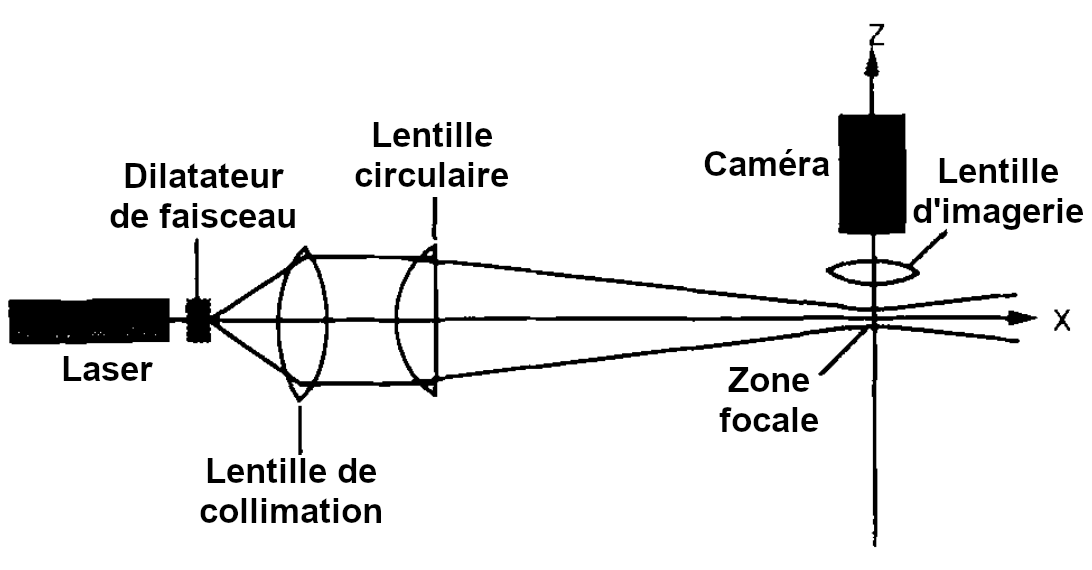
\includegraphics[width=\textwidth]{\Figures/light_sheet.png}
       \caption{
            \label{fig:light}
            Principe de fonctionnement d'un microscope à feuille de lumière.
            \newline
            Une lentille circulaire permet de créer une feuille de lumière au niveau de la zone focale.
            En plaçant l'échantillon au sein de cette feuille de lumière, il est alors possible de diminuant la quantité de lumière traversant l'échantillon, ce qui réduit la photo\hyp{}toxicité. 
            \newline
            Traduction d'une figure provenant de Voie et al, 1993~\cite{voie_1993}.
            }
\end{figure}

%%
Cette approche présente plusieurs avantages. En illuminant l'ensemble du plan en une seule fois, il est possible d'acquérir le signal avec une caméra avec une rapidité supérieure aux scanners qui captent la lumière point par point.
Cela réduit considérablement la photo-toxicité et le photo\hyp{}blanchiment, ce qui est particulièrement avantageux pour les observations  \textit{in vivo}.
%
De nombreuses améliorations sont apparues au fil du temps, comme par exemple des feuilles de lumière plus homogènes obtenues grâce à l'emploi de deux sources opposées~\cite{huisken_2007}, ou bien l'emploi de deux objectifs.
%
Cependant, l'utilisation de la nappe de lumière limite la pénétration en profondeur dans l'échantillon, ainsi que la taille du champ d'acquisition, ce qui oblige à des acquisitions chevauchantes et des opérations de stitching des images très lourdes). Enfin, cette méthode génère des images de taille considérable (typiquement 1 To par image), ce qui entraîne donc des opérations informatiques très lourdes, pour le transfert, l'archivage et le traitement des images.

    \subsection{La microscopie confocale, la méthodologie la plus adaptée au \hcs{}}
    
Deux stratégies  permettent de faciliter l'acquisition de \pz{} en grand nombre: l'utilisation de cuves contenant les échantillons, ou l'utilisation de capillaires.
   
%% Acquisition par moules dans des plaques
%
Il est possible de faciliter l'acquisition du \pz{} par deux approches:
Assurer une régularité de placement entre les échantillons,
pour pouvoir paramétrer plus facilement le système d'imagerie, et assurer l'orientation des échantillons.
%%
%
La première approche consiste à utiliser des plaques standardisées (par exemple avec 96 puits)qui possèdent des espacements réguliers. Un échantillon est placé dans chaque puits, puis l'ensemble du puits est imagé. Cette stratégie permet des procédures robotisées permettant de multiplier le nombre d'échantillons gérés simultanément.
%
Cependant, cette approche impose d'effectuer des images bien plus grande que l'objet d'intérêt et une grande partie des images ne contiennent donc pas d'information. Souvent, la grande taille de la zone d'acquisition rend impossible le développement d'imagerie à aute résolution.

%%
%
\label{sec:moule_montage}
La seconde approche implique l'utilisation de moules de montage.
%
On peut soit utiliser des moules permettant de créer des puits dans un moule dans lesquels les échantillons seront insérés~\cite{donoughe_2018,kleinhans_2019}, soit à er des moules pour créer des pièges faisant appel à la microfluidique pour contraindre les échantillons~\cite{khalili_2019}. Dans les deux cas, l'orientation des échantillons peut être déterminée.
%
De plus, les systèmes de créations de puits ont été couplés avec l'utilisation de plaques standardisées~\cite{wittbrodt_2014}.
%
Il est ainsi possible de coupler les avantages des deux approches afin de limiter la zones d'imagerie et en ayant des échantillons présentant l'orientation désirée.

%% Vast
\label{sec:vast}
Le Vertebrate Automated Screening Technology bioimager~\cite{pardomartin_2010} (VAST) est la méthode de robotisation d'acquisition d'images de \pz{} par capillaire la plus représentée dans la littérature~\cite{jarque_2018,teixid_2019}. Il permet d'imager des échantillons entre 2 et 4 dpf.
%
Ce système est un accessoire à associer à un microscope droit ou inversé, que ce soiet des microscopes à epifluorescences, des microscopes confocaux ou des microscopes à disque rotatif~\cite{early_2018, guo_2017}.
%
Le VAST est un système de pompes et de moteurs permettant d'aspirer des larves de \pz{} dans un capillaire, dont une partie en verre est placée sur la platine du microscope. 
%
Il est possible de faire tourner le capillaire afin d'assurer l'orientation désirée de l'échantillon.
%
Cet outil permet donc de faciliter l'imagerie du \pz{} en assurant la qualité de positionnement des échantillons.

%%
%
Il est possible de réaliser un chargement manuel des échantillons ou bien d'utiliser un robot de chargement des échantillons permettant de pipeter automatiquement des échantillons qui se trouvent dans une plaque de culture cellulaire (ayant jusqu'à 96 puits).
%
Cependant, ce système, lourd à mettre en oeuvre, est de plus relativement fragile, et requiert une longue expertise du système pour être fiable.
De plus, l'utilisation de capillaires induit des aberrations optiques en dehors du centre du capillaire ce qui empêche l'obtention d'images 3D sans aberration sur les côtés et donc par exemple toute analyse volumétrique. Enfin, l'utilisation de capillaires limite la gamme de diamètres des échantillons, les juvéniles ne pouvant par exemple par être observés.

\end{document}
